% Introduction
\section{Introduction}
%%
\iffalse
Main components in this section:

\textbf{1.The significance of this research and the background:}
\vspace{3mm}

\textbf{2.The weakness of the existing methods and the challenges:}

The existing methods can be divided into two categories :  deterministic or probabilistic.

The deterministic approaches assume there are no collision or are only suitable for two nodes.
Some assume all the nodes are the neighbor of each other.

Some methods assume nodes have an estimate of $N$, which is the total amount of sensors in the network.

The probabilistic approaches have a poor performance and can not guarantee a worst case bound. 


Challenge of my work:
We consider the most demanding problem model in this work, which is also closest to the practical situation.

\textbf{3.The main contribution and the key idea of my work:}

Consider the partially-connected network, which is the most demanding problem model.

Assume nodes do not have an estimate of $N$.

Combine the advantages of both two category approaches.

The Proposed algorithm guarantees achieving neighbor discovery within $O(nf(\theta))$, which holds a better
performance than the state-of-the-art works.

The core is to propose a deterministic approach to  align the sensors' wake-up time and then achieve neighbor discovery with a probabilistic approach.
\fi
%%
%Picture1: 	热力图:说明网络中nodes的分布关系
%Picture2:	邻居图:说明邻居的连接时部分连接的

%********************start:

%keywords: partially-connected networks,
%energy-efficient networks: global & local duty circle
%nodes distribution
%combine the deterministic and probabilistic advantages.

 %Background application:
Information and Communication Technology (ICT) equipment  
has exploded on the scene in the last twenty years\cite{zeadally2012energy}. 
Varying from their specific applications, these devices consists of a wide variety of networks.


%Theme&&main topic: Neighbor discovery
Neighbor discovery is a fundamental means for the devices 
to participate in network communication.
%introduction the existing  methods and their weakness
A popular way to deal with this issue is to construct a deterministic 
sequence of transmission state in each time slot
\cite{wang2015blinddate,qiu2016talk,dutta2008practical,
sun2014hello,bakht2012searchlight,chen2015heterogeneous,kandhalu2010u}. 
It holds an obvious advantage that the time to discovery a neighbor 
node can be bounded within a limited time. 
Nevertheless, most deterministic approaches only consider two 
nodes to discover each other, without further deliberating on the details 
(e.g. collisions from neighbors) when applying for multi-nodes.
Instead, there are some probability based algorithms showing an ideal expected time 
bound for multi-nodes to find their neighbors. However, the weakness part 
of this kind of methods lies in the poor performance of discovery latency in the worst case.





%this paper focus on two points 


%Partially-Connected Networks: Background&motivation&contribution 
%Why Partially-Connected Networks is a practical assumption


%why we consider partially-connected networks
A more crucial issue is that neither deterministic or probabilistic approaches 
consider a partially-connected networks in reality, 
the devices of which can only possess a fraction neighbors among all the nodes.
Deploying a fully-connected network in a large-scale area, 
such as campus networks, wireless sensor networks,
mobile gaming community, etc., is technically impractical 
due to the limited sensing range of devices communication.
How far the other nodes can be detected as a neighbor for a mobile equipment  
depends on criterion such as the received signal strength.
Thus a practical situation is that in a network , the nodes are partially connected with its  
detectable neighbors.


\vspace{3mm}
 *********To be dealt with details later********
 
 
\textbf{How we deal with partially-connected networks:}

1. Consider distribution of network devices: uniform distribution normal distribution

2. propose a distribution based Alano alogrithm

*

*

*

*

\begin{figure}[!t]
\centering
\subfigure[Normal distribution density function]{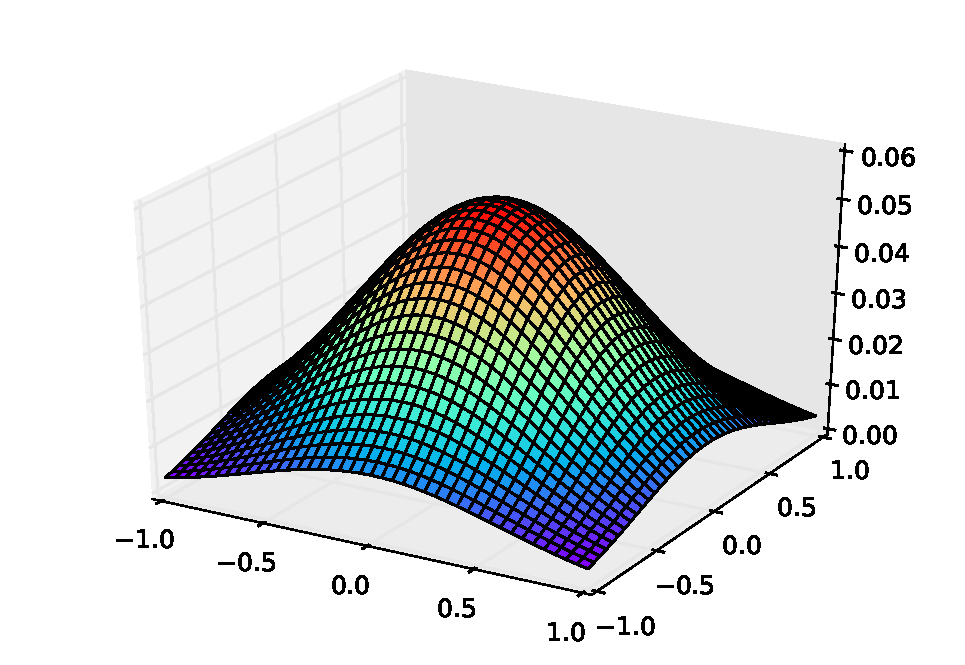
\includegraphics[width=2.5in]{./Figure/normalDistribution.eps}}
\vspace{0.03in}
\subfigure[Network obeys normal distribution  ]{\includegraphics[width=2.5in]{./Figure/normalProject}}
\caption{An example of a network obeying normal distribution.}
\label{NDexample}
%\vspace{-0.2in}
\end{figure}


\textbf{*Motivation of energy-efficient networks:}

%Energy-Efficient Networks: Background&motivation&contribution


Among the partially-connected networks, there is a special 
one named energy-efficent network.
Nodes in this type of networks have to maintain 
strict power budgets to attain years of lifetime\cite{dunkels2011contikimac}.
Duty circle mechanism, the , is utilized to power-awareness ought to be fully taken into consideration.
Correspondingly, the neighbor discovery process needs adjustment to deal with the dilemma between 
a balance of energy-efficiency and low- latency.


\textbf{Contribution conclusion}

In this paper, we first focus on the mathematical analysis of the distribution of the nodes in the networks.
We give a expectation of neighbor number for each node in a network which obey****
  propose Alano\footnote{Alano is the god of luck in Greek mythology }, 
a RDS-Alano algorithm for partially-connected networks 
as well as a TP-Alano algorithm for the energy-effienct networks.




%power-awareness is fully taken into consideration in the design, implementation, deployment, and maintenance of ICT technologies. 


%we use the technique to aline the wake-up slot and invoke the proposed 
%第二章介绍现有模型和算法的缺陷

%the advantage and disadvantage of D&P and why they can be combined.



%本文的贡献
The contributions of this paper are as follows:
%In this paper, we propose a new method to construct sequence
%we propose improved algorithms for both scenarios and our contributions are as follows:
\begin{itemize}
\item[1)] We model the distribution of nodes in their networks and analyse the 
expectation number of neighbors of a node in uniform distribution and normal
distribution and then propose Alano, a strategy
\item[2)] We propose a Relaxed DifferenceSet based Alano algorithm (RDS-Alano) 
for the global duty circle scenario. 
\item[3)] We propose a Traversing Pointer based Alano algorithm (TP-Alano) 
for the local duty circle scenario. 
\end{itemize}

\textbf{*Rest part structure}

%后文的结构
The remainder of the paper is organized as follows.
The next section highlights some related work and 
puts forward some serious problems. 
Some notion definitions and the system model are given in Section
\ref{sectionmodel}. 
We analyse the node's expectation number of neighbors and 
propose Alano algorithm in \ref{PCN} as a foundation.
Section \ref{EEN} describes the RDS-Alano algorithm for global
duty circle scenario and TP-Alano algorithm for local duty circle scenario
respectively in energy-efficient networks.
We have conducted extensive simulations, and the results are shown in Section
\ref{Evaluation}. Finally, we conclude the paper in Section
\ref{Conclusion}.


